\begin{flushleft}
Lorsque l'on ne souhaite pas s'initier à la programmation à proprement parler, il est possible d'utiliser Tinkercad pour créer ses programmes en passant par des algorithmes. Par ailleurs Tinkercad permet aussi de simuler vos montages pour être sûr qu'ils fonctionneront correctement lorsque vous les réaliserez avec votre carte.\vspace{0.2cm}
\end{flushleft}

\begin{flushleft}
\textbullet \, Se rendre sur le site : \url{https://www.tinkercad.com/} et cliquer sur \textit{Rejoindre maintenant} :
\end{flushleft}

\begin{figure}[!h]
    \centering
    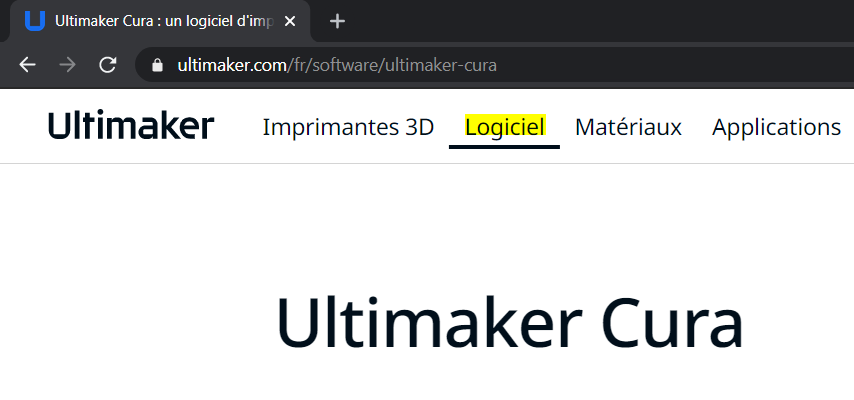
\includegraphics[width=475pt,height=150pt]{Déroulé/Jour_3/configuration Tinkercad/étape1.PNG}
    \caption{Configuration Tinkercad - \'Etape 1}
    \label{fig:my_label}
\end{figure}

\begin{flushleft}
\textbullet \, Une fois votre compte créé, cliquer sur \textit{Circuits} :
\begin{figure}[!h]
    \centering
    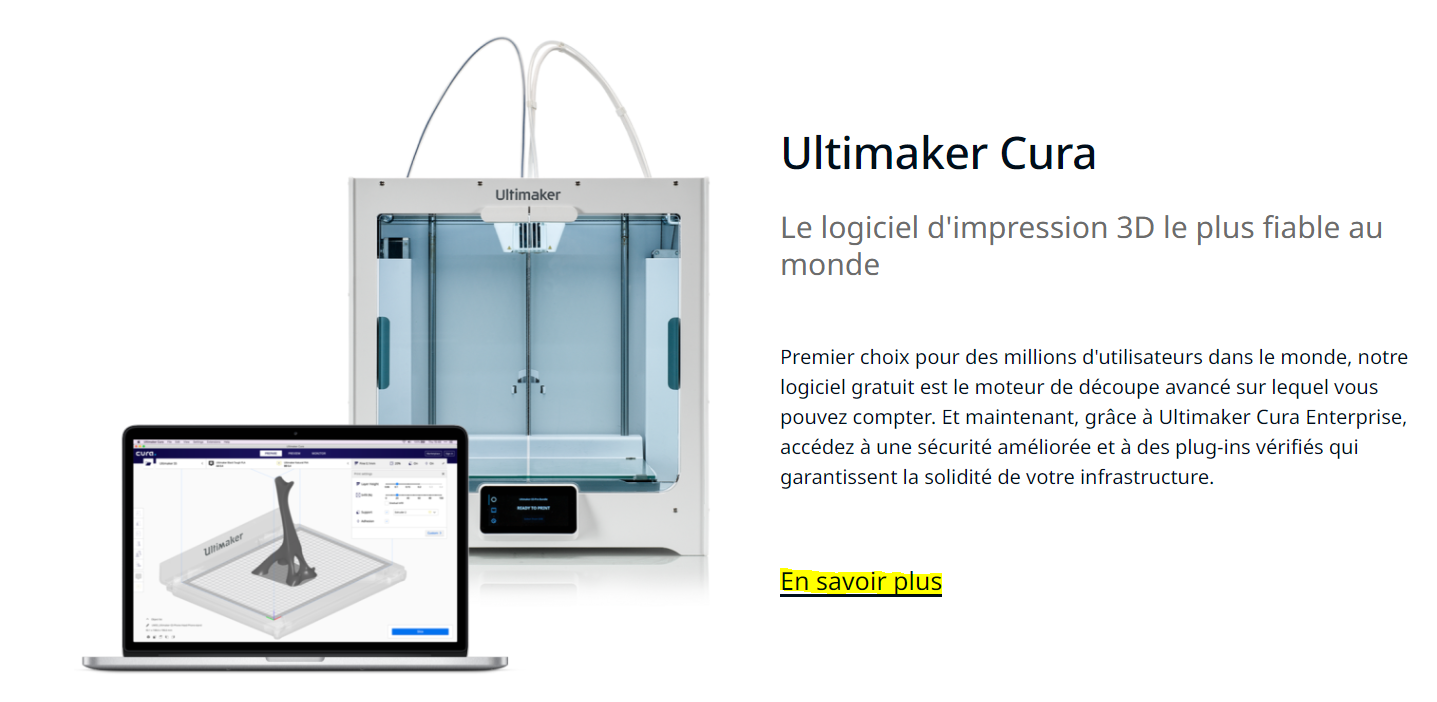
\includegraphics[width=150pt,height=150pt]{Déroulé/Jour_3/configuration Tinkercad/étape2.PNG}
    \caption[\'Etape 2]{Configuration Tinkercad - \'Etape 2}
    \label{fig:my_label}
\end{figure}

%provisoire
\newpage

\textbullet \, Cliquer sur \textit{Créer un ciruit} :
\begin{figure}[!h]
    \centering
    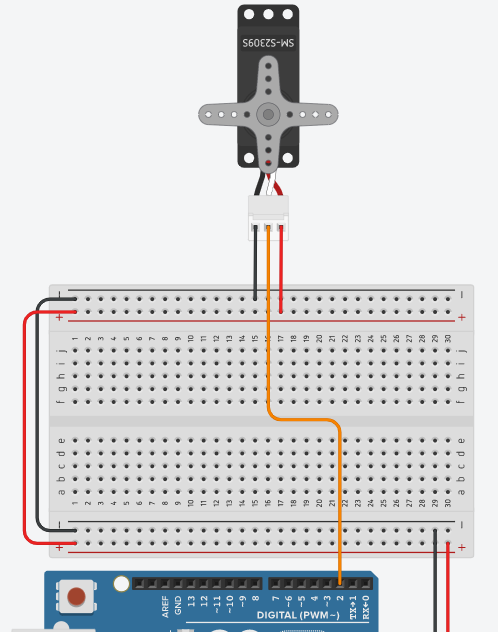
\includegraphics[width=150pt,height=100pt]{Déroulé/Jour_3/configuration Tinkercad/étape3.PNG}
    \caption[\'Etape 3]{Configuration Tinkercad - \'Etape 3}
    \label{fig:my_label}
\end{figure}

\textbullet \, Cliquer sur la petite flèche :
\begin{figure}[!h]
    \centering
    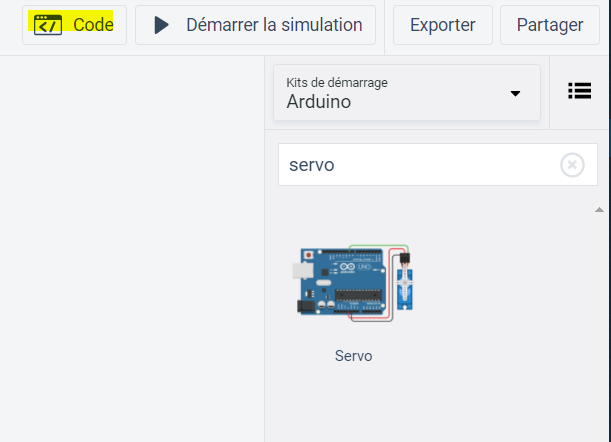
\includegraphics[width=450pt,height=100pt]{Déroulé/Jour_3/configuration Tinkercad/étape4.PNG}
    \caption[\'Etape 4]{Configuration Tinkercad - \'Etape 4}
    \label{fig:my_label}
\end{figure}

\textbullet \, Aller dans \textit{Kits de démarrage}, sélectionner \textit{Arduino} et choisir la \textit{Platine d'essai} :
\begin{figure}[!h]
    \centering
    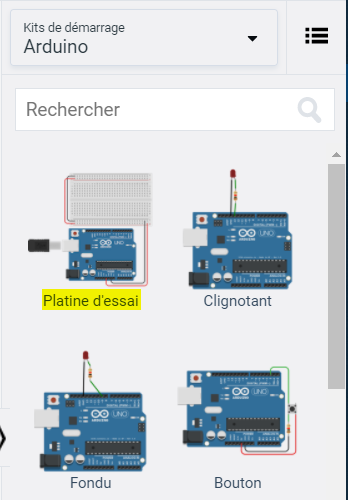
\includegraphics[width=200pt,height=250pt]{Déroulé/Jour_3/configuration Tinkercad/étape5.PNG}
    \caption[\'Etape 5]{Configuration Tinkercad - \'Etape 5}
    \label{fig:my_label}
\end{figure}

%provisoire
\newpage

\textbullet \, Déposer la platine d'essai sur la surface de travail :
\begin{figure}[!h]
    \centering
    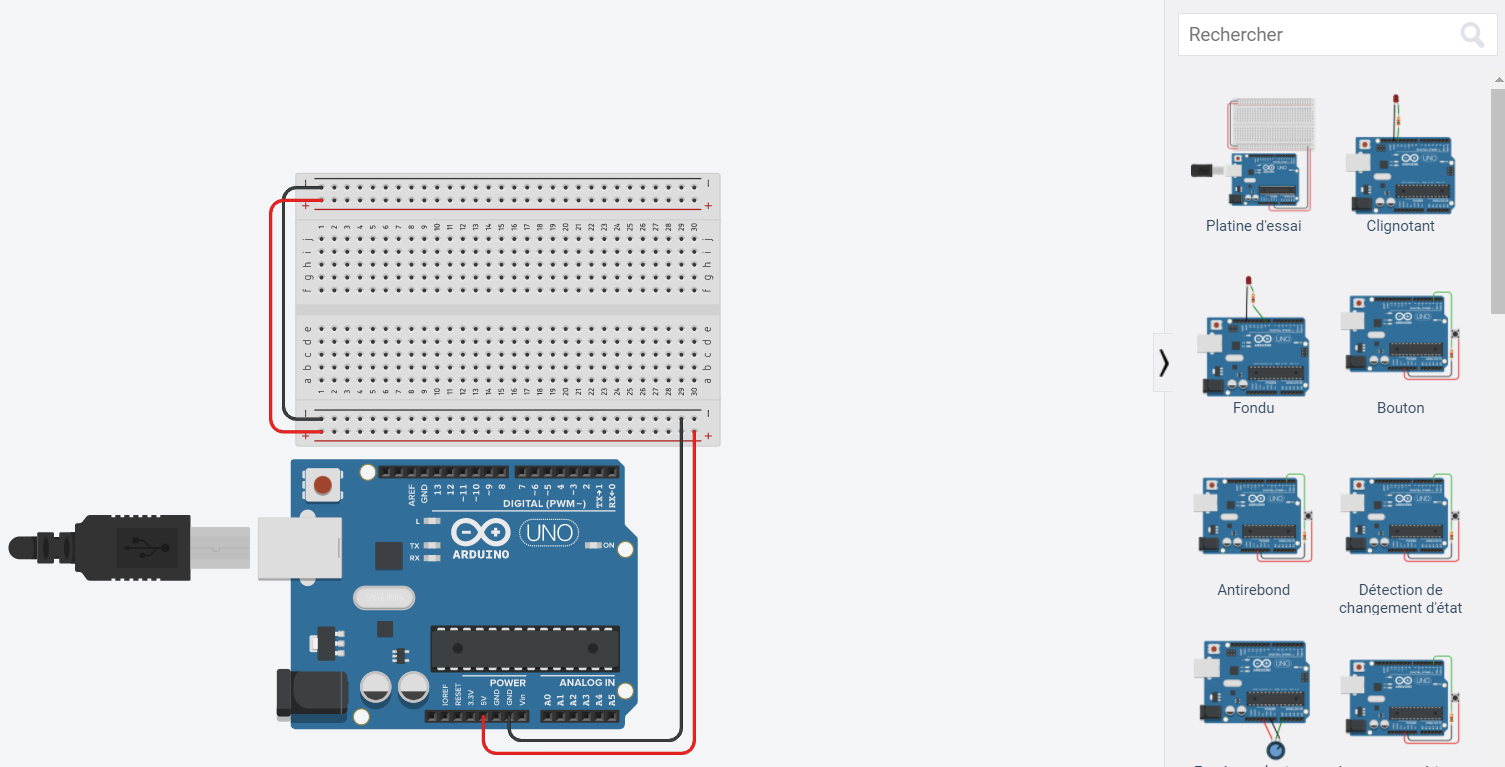
\includegraphics[width=300pt,height=125pt]{Déroulé/Jour_3/configuration Tinkercad/étape6.PNG}
    \caption[\'Etape 6]{Configuration Tinkercad - \'Etape 6}
    \label{fig:my_label}
\end{figure}
\end{flushleft}